\section{SD kort modul}

SD kort modulet er ikke implementeret i denne endelige iteration af projektet.\\


Skærmmodulets hardware indeholder en SD kortholder i dettes shield. Denne holder kan tilgås med SPI forbindelser fra PortB input-/outputpins på Atmega2560 

\subsection{Datalogning}
 
SD kortet indrages i projektet med henblik på datalogning, hvilket udvider realtids spektrogrammets implementeringsmuligheder. Med datalogning vil det grafiske display ikke blive den eneste mulighed for at gengive lydkarakteristika. Mikrofon-dataen, som behandles til grafisk gengivelse, vil blive gemt på SD kortet i en tekstfil og kan derved behandles og analyseres senere, som kommasepareret fil. Hver logning består af et array med 128 elementer af 8 bit, hvilket vil blive logget i takt med at skærmen opdateres.

\subsection{Driver Implementering}

Med henblik på at implementere SD kort driveren på et lavt abstraktionsniveau i kode, så er der taget udgangspunkt i Simple FAT and SD Tutorial fra http://codeandlife.com [31-05-2018] med særlig henblik på del tre og fire.\\
Dette udgangspunkt er også valgt da SD kortets størrelse skal være minimal til at holde på logningsfilerne, og der implementeres FAT16 filsystem på SD kortet. FAT16 står for File Allocation Table og er et fungerende filsystem for SD kort under 2 GB størrelse.\\
Den implementerede kode er modificeret fra ovenstående guide, hvor der var et FAT16 bibliotek tilhørende, og kommunikerer med SD kortet på SPI protokolniveau, hvor SD kortet modtager kommandoer i størrelsen af seks byte. SD kortet svarer på disse kommandoer med en til fem byte. 

\begin{figure}[H]
	\center
	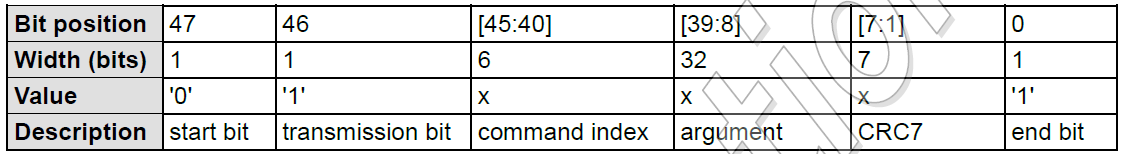
\includegraphics[width=1.0\textwidth]{Figur/SDcmd.png}
	\caption{SD SPI kommandoer fra Part1\_Physical\_Layer\_Simplified\_Specification\_Ver6.00}
	\label{fig:SDcmd}
\end{figure}

SD kort driveren kunne ikke implementeres til at være brugbar, hvilket kan ses under modultest SD kort driver. Koden kan forefindes i codeLifeTest mappen under Source\_code

